
\section{Asymptotic Distributed Consensus Algorithm}

The averaging consensus problem can be solved not only by DAC algorithms,
but also in many other ways, such as flooding, gossip and so on. In
the flooding algorithm, each sensor maintains a table of all sensors
values which initialize by its local value. At each iteration of the
flooding algorithm, every node exchanges the table with their neighbors.
After enough steps, which is larger than the diameter of the network.
Every node will get all the initial value of all nodes. Gossip algorithms
are asynchronous. Only one random node wakes up and randomly chooses
another node. The two nodes exchange their estimates and update to
the average of the two. 

Due to the simplicity and robustness of asymptotic distributed consensus
algorithm, it plays an important role in the practical problems. They
are already applied to network with a large number of nodes and proofed
to be robust against the topology variation. Once the network graph
is strong connected, the convergence to global consensus value is
guaranteed \cite{Ren2007}. In this section, we start from the first-order
DAC algorithm and then expand the algorithm to higher-order in order
to yields a higher the convergence rate.


\subsection{\label{sub:DT-First-Order-DAC}Discrete First Order Distributed Consensus
Algorithm}

First Order Distributed Consensus Algorithm (FO-DCA) update the local
value of node $i$ iteratively at each time-step $k$ by a weighted
sum of node\textquoteright{}s local values one time step before, given
by 

\begin{eqnarray}
x_{i}(k+1) & = & x_{i}(k)+\sum_{j\in\mathcal{N}_{i}}w_{ij}\left[x_{j}(k)-x_{i}(k)\right]\label{eq:1st iter. ni}\\
 & = & w_{ii}x_{i}(k)+\sum_{j\in\mathcal{N}_{i}}w_{ij}x_{j}(k)
\end{eqnarray}
where $k=0,1,2,...$ is the time index, $w_{ij}$ is the weight to
$x_{j}$ at node $i$, $w_{ij}=0$ if $(i,j)\notin\mathcal{E}$. Note
that we define a weight to node $i$ itself $w_{ii}=1-\sum_{j\in\mathcal{N}_{i}}w_{ij}$,
so that the sum of all weights equals to one, $\sum_{j=1}^{n}w_{ij}=1$. 

The iteration \prettyref{eq:1st iter. ni} can be written in a vector
form 

\begin{equation}
\mathbf{x}(k+1)=W\mathbf{x}(k)\label{eq:first order matrix}
\end{equation}
where $W$ is a weight matrix which refer to as the Perron matrix
induced by ${\cal G}$ \cite{Olfati-Saber2004}. This linear iteration
implies that $\mathbf{x}(k)=W^{k}\mathbf{x}(0)$ for $k=1,2,\cdots$. 

Since the initial value vector is randomly chosen, the matrix $W$
must satisfy some convergence conditions to make sure the iteration
convergent, and the convergence rate depends on the spectral radius
of matrix $W$.


\subsubsection{Convergence Conditions}

For the matrix iteration defined in \prettyref{eq:first order matrix},
the average consensus problem is to choose the weight matrix $W$,
so that for any initial value $\mathbf{x}(0)\in R^{n}$, $\mathbf{x}(k)$
converges to the vector 

\begin{equation}
\mathbf{\bar{x}}=\left(\mathbf{1}^{\mathrm{T}}\mathbf{x}(0)/n\right)\mathbf{1}=\dfrac{\mathbf{11}^{\mathrm{T}}}{n}\mathbf{x}(0)
\end{equation}

\begin{thm}
\cite{Xiao2004}\textup{\label{thm:convergence condition}$\lim_{k\rightarrow\infty}\mathbf{x}(k)=\mathbf{\bar{x}}$}
if and only if the matrix $W$ satisfie\textup{s
\begin{equation}
\lim_{k\rightarrow\infty}W^{k}=\dfrac{\mathbf{11}^{\mathrm{T}}}{n}.\label{eq:convege condition W}
\end{equation}
}Eq.\prettyref{eq:convege condition W} holds if and only if
\begin{eqnarray}
\mathbf{1}^{\mathrm{T}}W & = & \mathbf{1}^{\mathrm{T}}\label{eq: Converge condition W_Left}\\
W\mathbf{1} & = & \mathbf{1}\label{eq: Converge condition W_right}\\
\rho\left(W-\mathbf{11}^{\mathrm{T}}/n\right) & < & 1\label{eq:Converge cond. rhu<1}
\end{eqnarray}
where vector $\mathbf{1}=[1,1,\cdots1,]^{\mathrm{T}}\in R^{n}$, $\rho\left(\cdot\right)$
denotes the spectral radius of the matrix .
\end{thm}
Eq.\prettyref{eq: Converge condition W_Left} means that has a left
eigenvector $\mathbf{1}$ associated with the eigenvalue 1. This implies
that the sum of local value vector is not changed in the iteration
$\sum_{i\in\mathcal{V}}x_{i}\left(k+1\right)=\sum_{i\in\mathcal{V}}x_{i}\left(k\right)$
and the sum of each column of matrix $W$ is equal to one. Eq.\prettyref{eq: Converge condition W_right}
shows that $W$ is a row stochastic matrix and has an eigenvalue 1
with associated eigenvector $\mathbf{1}$. Both \prettyref{eq: Converge condition W_Left}
and \prettyref{eq: Converge condition W_right} together with the
convergence condition \prettyref{eq:Converge cond. rhu<1} means that
$W$ have a simple eigenvalue equals to one, and modular of all other
eigenvalues are less than one.
\begin{lem}
\textup{\label{thm:Share the eigenvalues}If $\lim_{k\rightarrow\infty}W^{k}=\dfrac{\mathbf{11}^{\mathrm{T}}}{n}$,
the matrix $W-\mathbf{11}^{\mathrm{T}}/n$ share the same eigenvalues
as matrix $W$ except the simple eigenvalue one is replaced by zero.}\end{lem}
\begin{proof}
Eq.\ref{eq: Converge condition W_Left} implies that the matrix $W$
has a left eigenvector $\mathbf{1}$ associated with eigenvalue one.
And Eq.\ref{eq: Converge condition W_right} implies that $\mathbf{1}$
is a right eigenvector of $W$ associated with eigenvalue one. The
fact that $\lim_{k\rightarrow\infty}W^{k}=\dfrac{\mathbf{11}^{\mathrm{T}}}{n}$
exists if and only if there exists a  matrix $U$ and $W$ can be
Jordan decomposition as 
\begin{equation}
W=U\left[\begin{array}{cccc}
J_{1}\\
 & J_{2}\\
 &  & \ddots\\
 &  &  & J_{m}
\end{array}\right]U^{-1}
\end{equation}
where $m$ is the number of distinct Jordan block. $J_{i}$ is the
$r_{i}$ dimensional Jordan block corresponding to eigenvalue $\lambda_{i}$,
$J_{1}=I_{r_{1}}$ is the $r_{i}$ dimensional identity matrix $\left(0\leq r_{i}\leq n\right)$
and all other Jordan block are convergent, i.e. $\rho\left(J_{i}\right)<1,2\leq i\leq m$.

Let $u_{1},u_{2},\ldots,u_{n}$ be the column of $U$ and $v_{1}^{T},v_{2}^{T},\ldots,v_{n}^{T}$
be row of $U^{-1}$. Then we have 
\begin{eqnarray}
\lim_{k\to\infty}W^{k} & = & U\left[\begin{array}{cc}
I_{r_{1}} & 0\\
0 & 0
\end{array}\right]U^{-1}\label{eq: W^k to infinity has Rank one}\\
 & = & \sum_{i=1}^{r_{1}}u_{i}v_{i}^{T}=\dfrac{\mathbf{11}^{\mathrm{T}}}{n}\label{eq:u*v=00003D11}
\end{eqnarray}
As the property of unitary matrix $U$, both $u_{i}$ and $v_{i}$
are set of orthogonal normal vectors, each $u_{i}v_{i}^{T}$ is a
matrix with rank one and matrix $\sum_{i=1}^{n}u_{i}v_{i}^{T}$ has
rank $n$. The sum $\sum_{i=1}^{r_{1}}u_{i}v_{i}^{T}$ must have rank
$r_{1}.$ Eq.\ref{eq:u*v=00003D11} shows that $r_{1}$ must equal
to one and $u_{i}v_{i}^{T}=\dfrac{\mathbf{11}^{\mathrm{T}}}{n}$,
both $u_{i}$ and $v_{i}$ are vectors with the same constant on all
components. Therefore, $W-\dfrac{\mathbf{11}^{\mathrm{T}}}{n}$ have
the same Jordan decomposition as $W$ except the Jordan block $J_{1}$
is replaced by zero, and all other Jordan block remain the same. This
completes the proof. 
\end{proof}
The convergence rate of the FO-DCA is related to the spectral radius
of matrix $W-\dfrac{\mathbf{11}^{\mathrm{T}}}{n}$. To get the maximum
convergence rate, an optimization problem to minimize the spectral
radius of the matrix could be solved \cite{Xiao2004}. 

\begin{equation}
\begin{array}{ccc}
\mbox{\mbox{Minimize }} & \rho\left(W-\frac{\mathbf{1}\mathbf{1}^{T}}{n}\right)\\
\mbox{Subject to } & \mathbf{1}^{\mathrm{T}}W=\mathbf{1}^{\mathrm{T}},\; W\mathbf{1}=\mathbf{1} & ,
\end{array}\label{eq: Opt. FO-DAC Problem}
\end{equation}
But it requires knowledge of network topology to solve the problem.
However, some non-optimal convergent weight matrices that satisfy
the condition in Eq.\prettyref{eq:convege condition W} are given
below. 


\subsubsection{First-order DAC Based On a Constant}

The simplest way to choose a weight matrix set all edges symmetric
and their weights equal to the constant $\epsilon$. A special weight
to a node itself is chosen to be $1-\epsilon\left|\mathcal{N}_{i}\right|$,
so that the sum of weights at a node is one. Therefore, the weight
matrix can be defined by the Laplacian matrix 
\begin{equation}
W=I_{n}-\epsilon L\label{eq:def. const FO-DAC}
\end{equation}
where the constant $\epsilon$ is the \textit{step length}. This kind
of DAC algorithm is called the \textit{constant FO-DAC}.

Let $\mathbf{e}_{1},\mathbf{e}_{2},\ldots,\mathbf{e}_{n}$ be the
eigenvectors of $W$ and $\lambda_{1}\left(W\right),\lambda_{2}\left(W\right),\ldots,\lambda_{n}\left(W\right)$
be the associated eigenvalues and they are ordered so that $1=\left|\lambda_{1}\left(W\right)\right|\geq\left|\lambda_{2}\left(W\right)\right|\geq\ldots\geq\left|\lambda_{n}\left(W\right)\right|$.
The largest eigenvalue $\lambda_{1}\left(W\right)$ is called the
\textit{dominant eigenvalue} and associated eigenvector $\mathbf{e}_{1}$
is called the \textit{dominant eigenvector}. 

From Eq.\prettyref{eq:def. const FO-DAC}, the eigenvalues of these
two matrix $W$ and $L$ have relationship given by $\lambda_{i}\left(W\right)=1-\epsilon\lambda_{i}\left(L\right)$.
Thus, we can determine the convergence range of $\epsilon$ in terms
of $\lambda\left(L\right)$.


\paragraph*{Choosing the step length}

For the constant FO-DAC algorithm, it is convergent, if and only if
the step length $\epsilon$ is in the range $\left(0,2/\lambda_{n}\left(L\right)\right)$.
And the optimal step length which maximize the convergence rate is
$\epsilon{}_{opt,FO}=\frac{2}{\lambda_{2}\left(L\right)+\lambda_{n}\left(L\right)}$
\cite{Xiao2004}. The boundary of the dominant eigenvalue $\lambda_{n}\left(L\right)$
can be found in \cite{Russell1994}, given by $d_{max}+1\leq\lambda_{n}\left(L\right)\leq\max\left\{ d_{u}+d_{v}\right\} $,
where $\left(u,v\right)\in{\cal E}$ , $d_{u}$ is the degree of node
$v_{u}$ and $d_{max}=\max_{v_{i}\in{\cal V}}\left|{\cal N}_{i}\right|$
is the maximum degree of nodes in the network. By Gerschgorin's theorem,
we have another upper boundary of $\lambda_{n}\left(L\right)\leq2d_{max}$,
then convergence is guaranteed if $\epsilon\in\left(0,1/d_{max}\right]$. 


\subsubsection{First Order DAC based on local degree}

Another option is Metropolis weight matrix (or local degree weight
matrix), where each weight is determined by degree of the two nodes
on the edge,

\begin{equation}
w_{ij}=\begin{cases}
\frac{1}{1+\max\left\{ d(i),d(j)\right\} }, & \mbox{if }(i,j)\in\mathit{\mathcal{E}}\\
1-\sum_{(i,k)\in\mathit{\mathcal{E}}}w_{ik}, & i=j\\
0, & \mbox{otherwise}
\end{cases}
\end{equation}
where $d(i)$ and $d(j)$ are the degrees of nodes $i$ and $j$. 

As shown above, the conventional DAC algorithm is depends on eigenvalues
of graph Laplacian matrix $\lambda_{i}\left(L\right)$ or degree of
nodes. However, in the section \ref{sub:Finite-time-Consensus-on},
we will show that the finite-time DAC algorithm in an invariant network
doesn't require these prior knowledge, if $\mathbf{x}\left(k\right)$
can be represented by a linear combination of a new normal basis defined
by eigenvectors of $W$. Thus, the weight matrix doesn't have too
much requirements and can be more easily chosen. This would be very
applicable because nodes in a distributed network usually doesn't
have any knowledge of network topology. 


\subsection{\label{sub:Discrete-High-Order}Discrete High Order Distributed Consensus
Algorithm }

Higher order Distributed Consensus Algorithm (HO-DCA) can have faster
convergence rate and potentially faster than FO-DCA. It can be easily
implemented by storing and using past data, and doesn't require additional
communication and network configuration. Moreover, HO-DAC can be regard
as a generalized form of distributed consensus algorithm \cite{Xiong2010}.
In \cite{Xiong2010}, the author assume all node can store and using
past data and define a topology-dependent matrix to update the initial
data. It involves more parameters than FO-DAC so that the optimization
problem has more degrees of freedom. When some parameters are set
to zero, the HO-DCA algorithm can reduce to the best constant FO-DAC
algorithm.

Since the convergence rate of the initial values is related to eigenvalues
of Laplacian matrix. In the optimization problem of HO-DCA, eigenvalues
of the associated graph Laplacian matrix or weight matrix must known. 

In a time-invariant, connected network, the $M-th$ high-order DAC
algorithm has the form:
\begin{eqnarray}
x_{i}(k) & = & x_{i}(k-1)-\epsilon\sum_{m=1}^{M}c_{m}(-\gamma)^{m-1}\Delta x_{i}(k,m),\label{eq:Iteration Second order x_i(k)}\\
\Delta x_{i}(k,m) & = & \sum_{j\in\mathcal{N}_{i}}\left(x_{i}\left(k-m\right)-x_{j}\left(k-m\right)\right),
\end{eqnarray}
Where $x_{i}(k)$ is the local value at node $i$ during iteration
$k$; $\mathcal{N}_{i}$ is the neighboring nodes set in which the
nodes can communicate reliably with node $i$; $\epsilon$ is a constant
step size; $M$ is the highest order number; $c_{m}$ are predefined
constants, where $c_{1}=1$ and $c_{m}\neq0\:(m>1)$; $\gamma$ is
a forgetting factor, such that $\left|\gamma\right|<1$. 

Define

\begin{equation}
\mathbf{x}(k)=\left[x_{1}(k),x_{1}(k),\ldots,x_{n}(k)\right]^{T}
\end{equation}
The Eq.\ref{eq:Iteration Second order x_i(k)} can be written in matrix
form

\begin{equation}
\mathbf{x}(k)=(I_{n}-\epsilon L)\mathbf{x}(k-1)-\epsilon\sum_{m=2}^{M}c_{m}(-\gamma)^{m-1}L\mathbf{x}(k-m)\label{eq:High Order Iter.Vec}
\end{equation}
where $L$ is the Laplacian matrix associated with the network graph.
assume $\forall k<0,\;\mathbf{x}(k)=\mathbf{x}(0)$, $\mathbf{x}(0)$
is the initial local state information for node $i$. The matrix form
states that when the forgetting factor $\gamma$ is set to zero, the
HO-DAC is reduced into the best constant FO-DAC algorithm given in 

Simulation result shows that, a higher order will have better convergence
rate, but should be trade off with the algorithm complexity and computational
cost. Also only a few improvement could be achieved if we introduce
larger than fourth order. 


\subsubsection{Convergence Rate Maximization Problem For HO-DAC}

Based on the iteration equation \ref{eq:High Order Iter.Vec}, the
$M-th$ high-order DAC algorithm in a time-invariant, connected and
undirected network, with initial local value vectors $\mathbf{x}(-M+1)=,\ldots,=\mathbf{x}(-1)=\mathbf{x}(0)$,
can be further defined by an $Mn\times Mn$ matrices
\begin{equation}
\mathbf{H}=\left[\begin{array}{cccc}
I_{n}-\epsilon L & c_{2}\gamma\epsilon L & \cdots & -c_{M}(-\gamma)^{M-1}\epsilon L\\
I_{n} & \mathbf{0}_{n\times n} & \cdots & \mathbf{0}_{n\times n}\\
\vdots & \ddots &  & \vdots\\
\mathbf{0}_{n\times n} & \cdots & I_{n} & \mathbf{0}_{n\times n}
\end{array}\right]
\end{equation}
\begin{equation}
\mathbf{J}=\left[\begin{array}{cccc}
\mathbf{K} & \mathbf{0}_{n\times n} & \cdots & \mathbf{0}_{n\times n}\\
\mathbf{K} & \mathbf{0}_{n\times n} & \cdots & \mathbf{0}_{n\times n}\\
\vdots & \vdots & \ddots & \vdots\\
\mathbf{K} & \mathbf{0}_{n\times n} & \cdots & \mathbf{0}_{n\times n}
\end{array}\right]
\end{equation}
 where $\mathbf{K}=\left(\frac{1}{n}\right)\mathbf{1}\mathbf{1}^{T}$,
and $\mathbf{0}_{n\times n}$ denotes the $n\times n$ all-zero matrix. 

The high-order DAC algorithm with initial condition $\mathbf{x}(-M+1)=,\ldots,=\mathbf{x}(-1)=\mathbf{x}(0)$
is convergent if and only if $\rho\left(\mathbf{H}-\mathbf{J}\right)<1$
\cite{Xiong2010}. Then a spectral radius minimization problem to
find the optimal $\epsilon$ and $\gamma$ for the high-order DAC
algorithm is formulated as

\begin{equation}
\begin{array}{cc}
\mbox{\mbox{Minimize }} & \rho\left(\mathbf{H}-\mathbf{J}\right)\\
\mbox{Subject to } & \epsilon,\gamma\in R
\end{array},\label{eq: High order spectral radius problem}
\end{equation}


As shown in Eq.\prettyref{eq: High order spectral radius problem},
the convergence rate maximization for high order DAC algorithm can
be cast into a spectral radius minimization problem. Finding the solution
is not easy due to we have to solve the high-order polynomial to calculate
eigenvalues. For example, the high-order polynomial of the eigenvalues
of $\mathbf{H-J}$ when $M=3$, $c_{1}=1$ and $c_{2}=1$ is 
\begin{equation}
f(\lambda)=\lambda^{3}-\left(1-\epsilon\lambda_{i}\left(L\right)\right)\lambda^{2}-\gamma\epsilon\lambda_{i}\left(L\right)\lambda+\gamma^{2}\epsilon\lambda_{i}\left(L\right)=0\label{eq: eigenvalue equation of H-J}
\end{equation}
where $\lambda_{i}(L)$ is the $i^{th}$ smallest eigenvalue of the
Laplacian Matrix \cite{Xiong2010}. 

Since each $\lambda_{i}(L),\; i=1,2,\cdots,n$ with generate one equation
which has $M$ roots, there are totally $M\times n$ eigenvalue for
$\mathbf{H-J}$. Then, problem Eq.\prettyref{eq: High order spectral radius problem}
can be written into minimize the maximum absolute value of all the
eigenvalues of $\mathbf{H-J}$. 
\begin{equation}
\begin{array}{cc}
\mbox{Minimize } & \mbox{max}\{\left|\lambda_{i}\left(\mathbf{H-J}\right)\right|\},\: i=1,2,\cdots,n\\
\mbox{Subject to } & \epsilon,\gamma\in R
\end{array},\label{eq:HO-DAC Opt. Problem}
\end{equation}



\subsubsection{Solve The Problem: Convergence rate maximization}

The convergence rate optimization problem \ref{eq:HO-DAC Opt. Problem}
of HO-DAC in undirected network can be graphically illustrated by
the \prettyref{fig:Find-minimum-rho(H)}, where the surface of $\mbox{max}\{\left|\lambda_{i}\left(\mathbf{H-J}\right)\right|\},\: i=1,2,\cdots,n$
is plotted and the optimal solution $\left(\epsilon{}_{opt},\gamma_{opt}\right)$
is marked with a star. We denote the optimized spectral radius by
$\rho_{opt}=\mbox{\mbox{min}}\rho\left\{ \left(\mathbf{H}-\mathbf{J}\right)\right\} $. 

Since the eigenvalues in the high-order polynomial \prettyref{eq: eigenvalue equation of H-J}
are network topology dependent, the solution of the problem \ref{eq:HO-DAC Opt. Problem}
may not have a unique analytical solution when the order is larger
than second. In this case, the problem will be solved numerically,
for example using steepest descent method. 

\begin{figure}
\hfill{}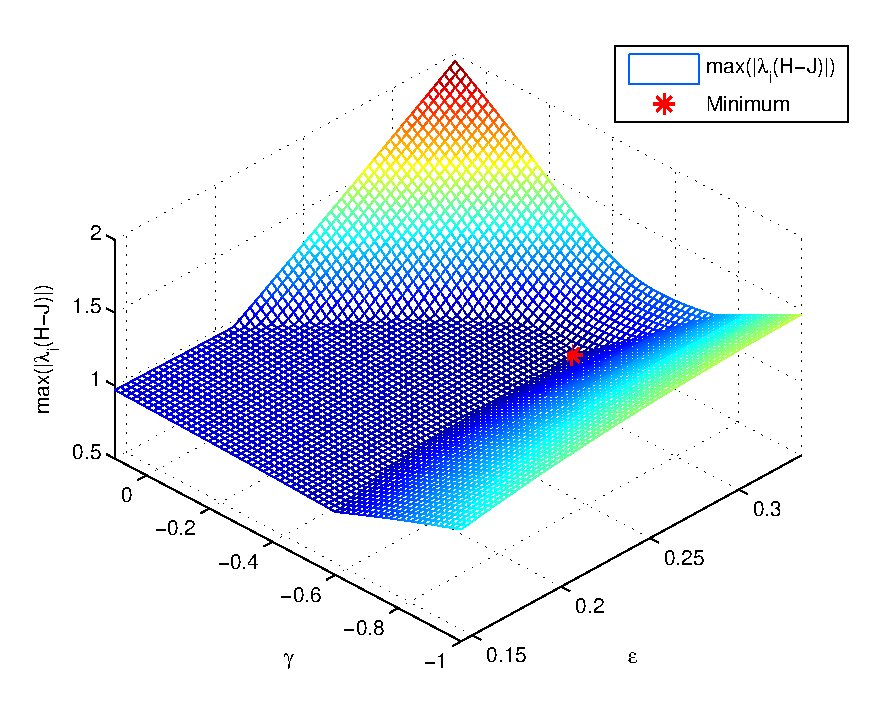
\includegraphics[height=9cm]{D:/Dropbox/PaperWork/FirstYearReport/Lyx_v/images/3order_max_lambda}\hfill{}\hfill{}\caption{\label{fig:Find-minimum-rho(H)} Illustration of Convergence rate
optimization, $\min\left\{ \mbox{max}\left[\lambda_{i}\left(\mathbf{H-J}\right)\right]\right\} ,\: i=1,2,\cdots,n$. }
\end{figure}


\begin{figure}
\hfill{}\includegraphics[height=9cm]{\string"Graph/Convergence region\string".pdf}\hfill{}\hfill{}\caption{\label{fig:Convergence-Region}Convergence Region for second order
DAC. }
\end{figure}


However, the second order DAC (SO-DAC), does exist an analytical solution.
As pointed out in \cite{Xiong2009a}, the convergence region for second
order DAC in undirected network which satisfy $\rho\left(\mathbf{H}-\mathbf{J}\right)<1$
is ${\cal R}={\cal R}_{1}\cup{\cal R}_{2}$, where 
\begin{eqnarray}
{\cal R}_{1} & = & \left\{ \frac{-1}{\epsilon\lambda_{n}\left(L\right)}<\gamma<1,0<\epsilon<\frac{1}{\lambda_{n}\left(L\right)}\right\} \\
{\cal R}_{2} & = & \left\{ \frac{-1}{\epsilon\lambda_{n}\left(L\right)}<\gamma<\frac{2}{\epsilon\lambda_{n}\left(L\right)}-1,\frac{1}{\lambda_{n}\left(L\right)}\leq\epsilon<\frac{3}{\lambda_{n}\left(L\right)}\right\} \label{eq:Def Convergence region R1 R2}
\end{eqnarray}
Fig.\ref{fig:Convergence-Region} graphically illustrate these region,
${\cal R}_{1}$ and ${\cal R}_{2}$ are defined in \prettyref{eq:Def Convergence region R1 R2}.
Note the dashed line separates the regions in which $\lambda_{n'}\left(\mathbf{H}\right),\lambda_{n"}\left(\mathbf{H}\right)$
are real and complex. In addition, optimal solution is always located
on this line. Moreover, the eigenvalues of $\mathbf{H}$ corresponding
to eigenvalue of $\lambda_{i}\left(L\right)$ is denoted by $\lambda_{i'}\left(\mathbf{H}\right)$
and $\lambda_{i"}\left(\mathbf{H}\right)$, which is 
\begin{eqnarray}
\lambda_{i'}\left(\mathbf{H}\right) & = & \frac{1}{2}\left[1-\epsilon\lambda_{i}\left(L\right)+\sqrt{\left(1-\epsilon\lambda_{i}\left(L\right)\right)^{2}+4\gamma\epsilon\lambda_{i}\left(L\right)}\right],\nonumber \\
\lambda_{i"}\left(\mathbf{H}\right) & = & \frac{1}{2}\left[1-\epsilon\lambda_{i}\left(L\right)-\sqrt{\left(1-\epsilon\lambda_{i}\left(L\right)\right)^{2}+4\gamma\epsilon\lambda_{i}\left(L\right)}\right].\label{eq:2nd-DAC lambda_H solution}
\end{eqnarray}
 

Since $\lambda_{2}\left(L\right)\leq\dots\leq\lambda_{n}\left(L\right)$,
in the convergence region of the second order DAC algorithm, the optimization
problem \prettyref{eq:HO-DAC Opt. Problem} can be equivalent to 
\[
\begin{array}{cc}
\mbox{Minimize } & \mbox{max}\{\left|\lambda_{2'}\left(\mathbf{H}\right)\right|,\left|\lambda_{2"}\left(\mathbf{H}\right)\right|,\left|\lambda_{n'}\left(\mathbf{H}\right)\right|,\left|\lambda_{n"}\left(\mathbf{H}\right)\right|\}\\
\mbox{Subject to } & \epsilon,\gamma\in R
\end{array},
\]


Finding the optimal solutions needs consideration of different combinations
of $\lambda_{2'}\left(\mathbf{H}\right),\lambda_{2"}\left(\mathbf{H}\right),\lambda_{n'}\left(\mathbf{H}\right),\lambda_{n"}\left(\mathbf{H}\right)$
when they are real value or complex value. However, for a connected
network, the $\lambda_{2'}\left(\mathbf{H}\right),\lambda_{2"}\left(\mathbf{H}\right)$
are real and $\lambda_{n'}\left(\mathbf{H}\right),\lambda_{n"}\left(\mathbf{H}\right)$
are complex values in the convergence region. When the minimum is
achieved, the following equation satisfied
\[
\left|\lambda_{2'}\left(\mathbf{H}\right)\right|=\left|\lambda_{n'}\left(\mathbf{H}\right)\right|=\left|\lambda_{n"}\left(\mathbf{H}\right)\right|
\]
Thus, by solving this equation, we have the optimal solution for second
order DAC algorithm.

\begin{eqnarray}
\epsilon{}_{opt,SO} & = & \frac{3\lambda_{n}(L)+\lambda_{2}(L)}{\lambda_{n}(L)\left[\lambda_{n}(L)+3\lambda_{2}(L)\right]}
\end{eqnarray}


\begin{equation}
\gamma_{opt,SO}=-\frac{\left[\lambda_{n}(L)-\lambda_{2}(L)\right]^{2}}{\left[\lambda_{n}(L)+3\lambda_{2}(L)\right]\left[3\lambda_{n}(L)+\lambda_{2}(L)\right]}
\end{equation}
These parameters could be floored to all sensors before the algorithm
start so that it converges faster.

Besides these results, we need to point out that the optimal solution
$\epsilon{}_{opt,SO}$ and $\gamma_{opt,SO}$ have the following relationship
\[
\gamma_{opt,SO}=\frac{\left[1-\epsilon{}_{opt,SO}\lambda_{n}\left(L\right)\right]^{2}}{-4\epsilon{}_{opt,SO}\lambda_{n}\left(L\right)}
\]
which implies the value under the square root in \prettyref{eq:2nd-DAC lambda_H solution}
is equal to zero, and $\lambda_{n'}\left(\mathbf{H}\right),\lambda_{n"}\left(\mathbf{H}\right)$
are all real values. Additionally, the optimal solution is located
just on the boundary of the regions where $\lambda_{n'}\left(\mathbf{H}\right),\lambda_{n"}\left(\mathbf{H}\right)$
is real and complex respectably, shown as dashed line in Fig. \ref{fig:Convergence-Region}. 


\subsection{Simulation and Algorithms Performance}

To test the performance of high-order DAC algorithm with different
orders, a simulation is carry out on 1000 random generated networks.
The methods and parameters of network generation are illustrated in
fig.\ref{fig:Net-N16-R0,3}. The algorithm's performance is evaluated
by the average spectral radius and average mean square error, shown
in \prettyref{fig:DAC-comparation}. 


\subsubsection{Random Network Generation}

The following is a simulation of network generation to show how the
wireless sensor networks is distributed. First, we randomly and uniformly
distribute a certain number of nodes in a unit square. Second, each
sensor randomly choose a local initial value has equally probability
density function. Finally, connect any two nodes if their satisfy
a certain communication constrains. 

\begin{figure}[h]
\hfill{}\subfloat[\label{fig:Net-N50-E200}]{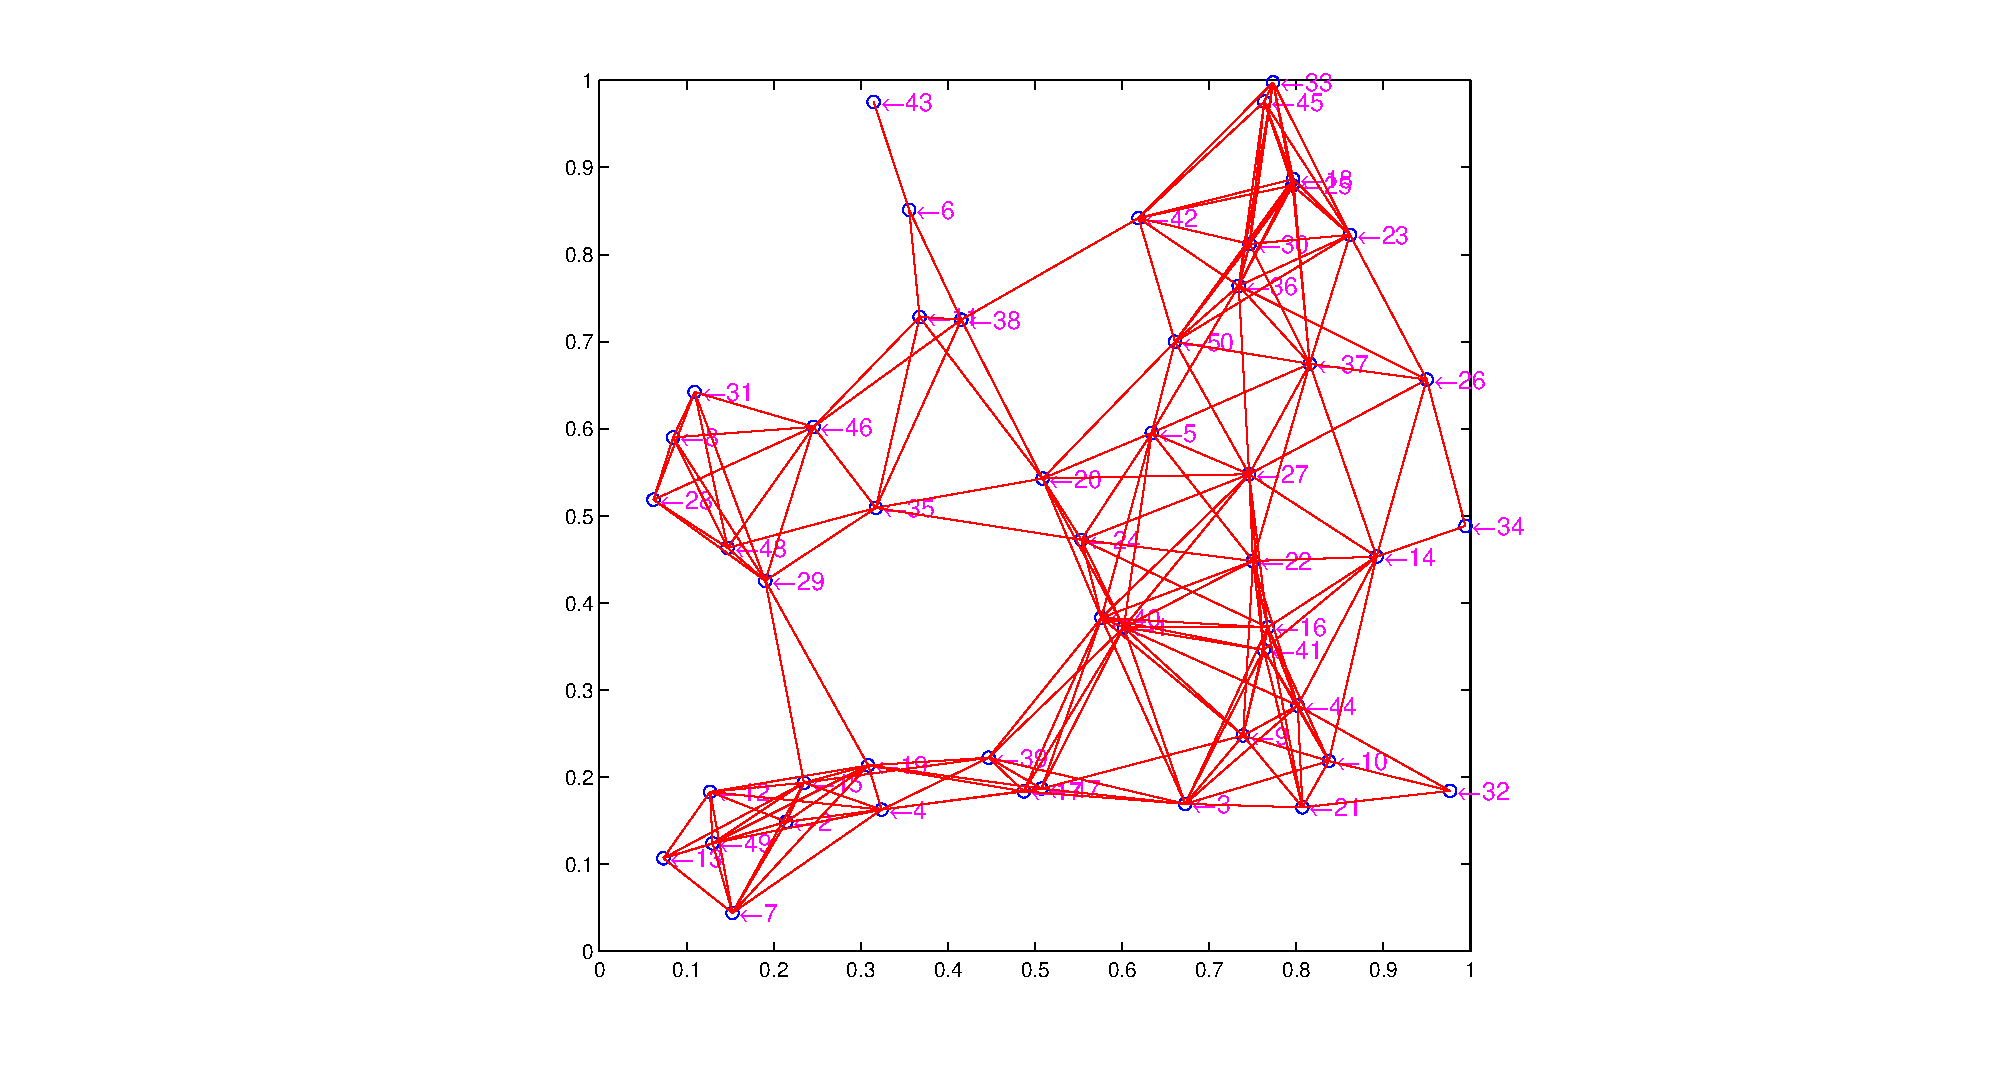
\includegraphics[width=7cm]{Graph/FirstYearReport/Lyx_v/images/Net50Edges200}

}\hfill{}\subfloat[\label{fig:Net-N16-R0,3}]{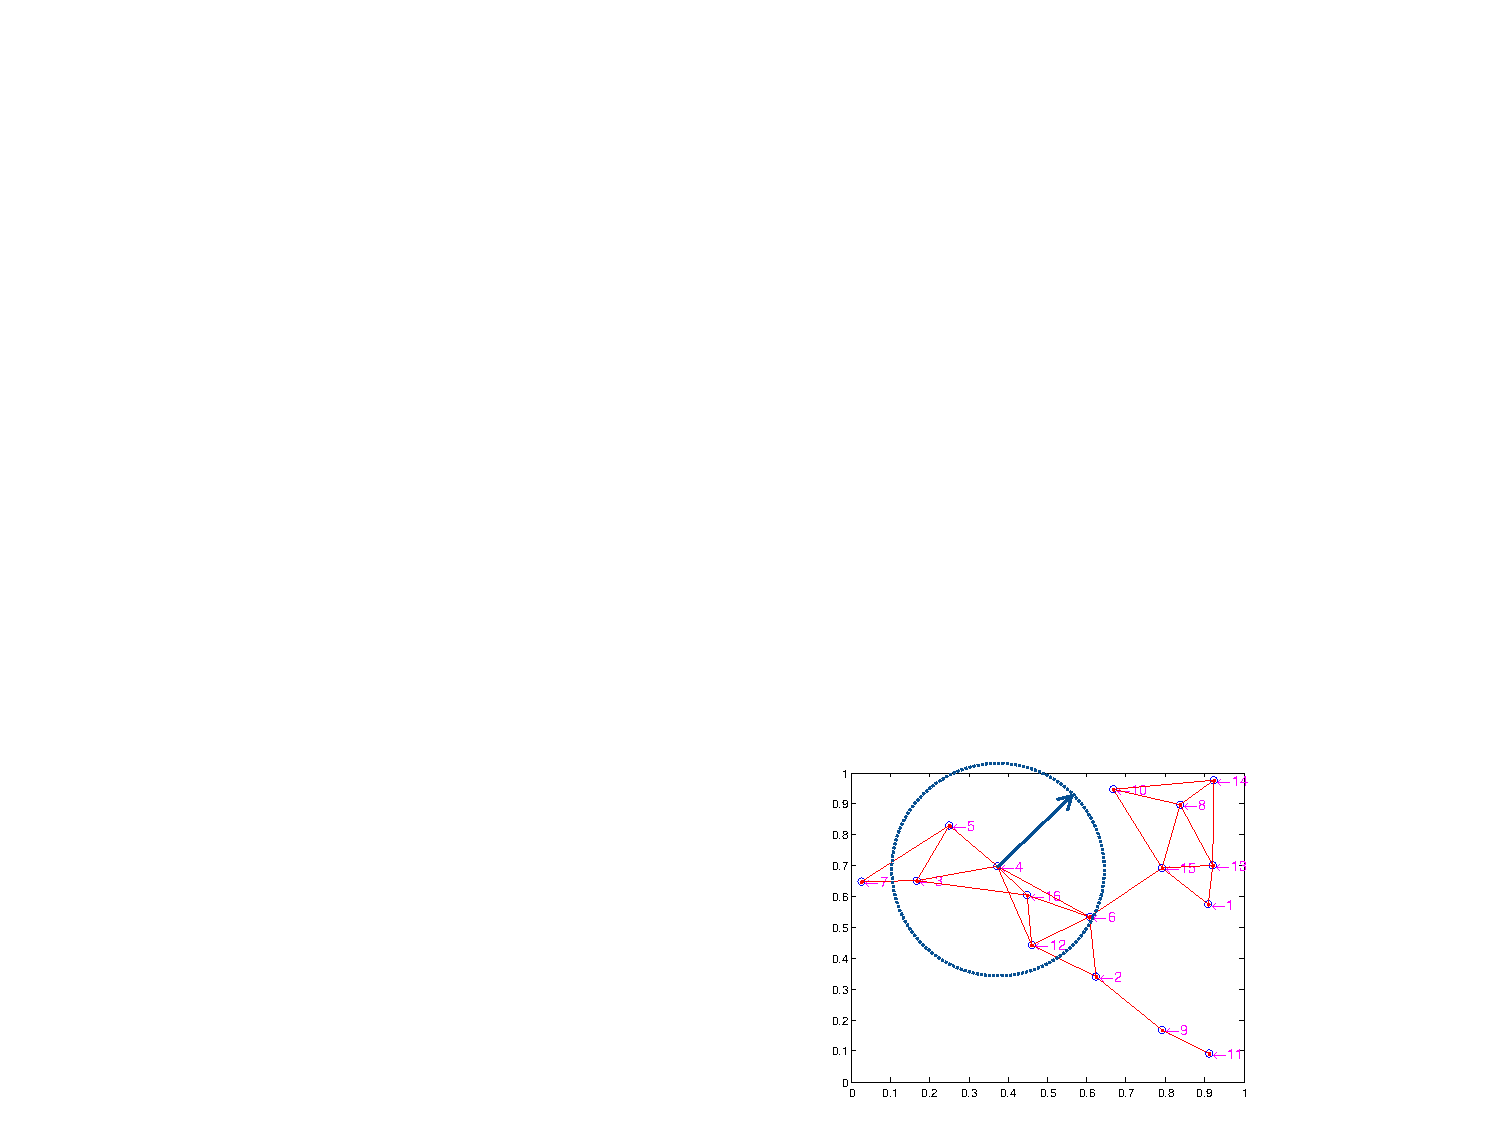
\includegraphics[width=7cm]{Graph/FirstYearReport/Lyx_v/images/Network_N16_R0,3}

}\hfill{}\caption{\label{fig:Random-Network}Randomly generated networks (a) 50 nodes
and 200 edges (b) 16 nodes and radius constrain $R=0.3$}
\end{figure}


There are some cases to generate the links between nodes.
\begin{casenv}
\item Consider the graph show in the Fig.\ref{fig:Net-N50-E200}, which
has 50 nodes and 200 edges.The number of nodes and edges are fixed;
50 nodes are randomly and uniformly distribute in the unit square;
a list that contains 200 shortest edges is created; Nodes are connected
if the edges belongs to the list. 
\item The network in Fig.\ref{fig:Net-N16-R0,3} is generating by connecting
any two nodes if their distance is less than the communication radius
constrain $R$. 
\end{casenv}

\subsubsection{Performance Comparison for Asymptotic DAC}

The figure.\ref{fig:DAC-SR-comp} shows the optimal spectral radius
for DAC algorithms with different communication radius constraints.
The performance for DAC algorithms with different orders are compared
by optimal spectral radius $\rho_{opt}=\mbox{\mbox{min}}\rho\left\{ \left(\mathbf{H}-\mathbf{J}\right)\right\} $,
which has the relationship with convergence rate given by $r_{opt}=-log\left(\rho_{opt}\right)$.
Y-axis is corresponding to the minimum spectral radius and x-axis
is corresponding to the radius constrain. For each instance of DAC
algorithm, the result is the minimum on the surface $\mbox{max}\{\left|\lambda_{i}\left(\mathbf{H-J}\right)\right|\}$
obtained by numerical searching. Each curve is the average of simulations
realized for 1000 instance of DAC initialized with random local value
vectors and random networks.

In another point of view, figure.\ref{fig:DAC MSE Compare} plots
the convergence behavior of mean square error of high-order DAC algorithms
together with first order DAC on random network. The MSE is defined
by 
\begin{equation}
MSE(k)=\frac{1}{n}\sum_{i=1}^{n}\left|x_{i}(k)-\bar{x}\right|^{2}.
\end{equation}
which Actually it is the Euclidean distance between current local
vector and the global average. shows the result when radius constrain
$R$ is $0.3$. In observing the gradient of curves, it is apparent
that higher-order DAC algorithm have larger convergence rate. However,
there are negligible improvement for the fourth order DAC compared
to the third order one. Furthermore, high-order DAC has a MSE overshoot
at the beginning. This phenomenon happens especially when communication
radius is small. Second order DAC algorithm does have a faster convergence
rate than first order algorithm as the slop of the curve is steeper.
But it become worse as it converge to error tolerance $10^{-6}$ more
later than the first order algorithm. Therefore, A hybrid algorithm
is proposed to overcome this disadvantage. Its step size and forgetting
factor are equal to the of first order DAC step size and second order
DAC forgetting factor respectively.

\begin{figure}
\hfill{}\subfloat[\label{fig:DAC-SR-comp} ]{\includegraphics[width=7cm,height=6.5cm]{\string"Graph/FirstYearReport/Lyx_v/images/Spectrum radius Compare_old_Ord1234\string".pdf}}\hfill{}\subfloat[\label{fig:DAC MSE Compare} ]{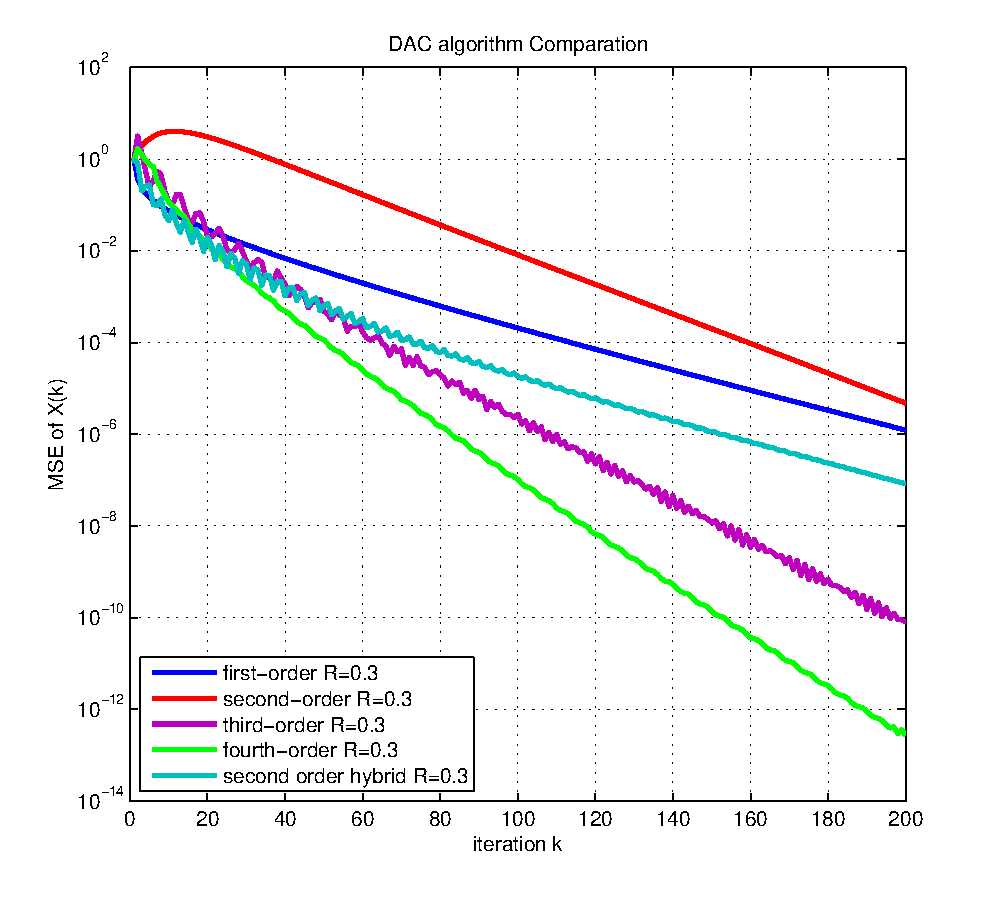
\includegraphics[width=7cm,height=6.5cm]{Graph/FirstYearReport/Lyx_v/images/DAC_Compr_ord1234&hybrid}

}\hfill{}

\caption{\label{fig:DAC-comparation}DAC algorithms comparison (a) compared
by spectral radius (b) compared by MSE}
\end{figure}

